
\documentclass[8pt]{article}
%	options include 12pt or 11pt or 10pt
%	classes include article, report, book, letter, thesis

\usepackage[a4paper,bindingoffset=0.2in,%
            left=0.6in,right=0.6in,top=0.2in,bottom=0.4in,%
            footskip=.15in]{geometry}
            
\usepackage[T1]{fontenc}
\usepackage[polish]{babel}
\usepackage[utf8]{inputenc}
\usepackage{lmodern}
\selectlanguage{polish}
\usepackage{blindtext}
\usepackage{pgfplots}
\usepackage{graphicx}


\title{Testowanie aplikacji .NET}
\author{Projekt 1 / Semestr 6\\ Aleksander Kosma\\grupa 2 tester-programista}
\date{14 Marzec 2018}

\begin{document}
\maketitle 

\section*{Dokumentacja projektu}
\subsection*{ Opis projektu}
Projekt obejmuje stworzenie biblioteki klas, przetestowanie biblioteki przy pomocy testów jednostkowych, oraz implementacja biblioteki w praktyce. Dodatkowo testy powinny zawierać w sobie wykorzystanie Data-Driven Unit Test, jak i wykorzystanie Microsoft Fakes( stuby i shimy).\\
Biblioteka klas ``BankSystem`` została stworzona z myślą o prostych symulacjach bankowych, głównie skupiając się na możliwości brania i spłaty kredytu. Biblioteka jest łatwa do modyfikacji pod względem warunków kredytu. Przy niskim nakładzie pracy można dodać bardziej skomplikowane warunki umowy. Mniejsze oprocentowanie w przypadku wcześniejszej spłaty, lub zmienna wartość kary za spóźnienie z opłatą.\\
\subsection*{ Diagram przypadków użycia}
Biblioteka umożliwia stworzenie prostego systemu bankowego. Możliwości systemu widoczne są na diagramie przypadków użycia:\\

\begin{center}
 \makebox[\textwidth]{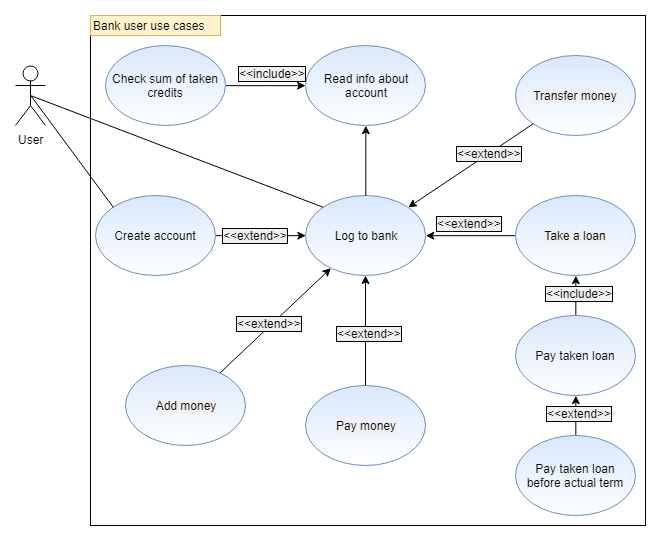
\includegraphics[width=18cm,height=12cm]{useCases.png}}
\end{center}
.\\
\\
\\
\\
\\
Zagłębiając się w opis poszczególnych funkcji:\\
\textbf{Stworzenie konta} - osoba może otworzyć konto w wybranym istniejącym systemie bankowym. Warunkiem koniecznym jest unikatowa nazwa konta, niewystępująca w danym banku.\\

\textbf{Logowanie} - osoba loguje się na konto za pośrednictwem banku w którym owe konto ma. Logowanie umożliwia użytkownikowi na pełne korzystanie z możliwości posiadania konta.\\

\textbf{Wyświetlanie danych} - osoba może wyświetlić swoje dane, sprawdzić wzięte kredyty, jak i ich pełną sumę.\\

\textbf{Przelew} - osoba może przelać pieniądze na inne konto. Do tej operacji potrzebna jest nazwa konta adresata. Adresat musi mieć konto w tym samym banku. Jeśli owy adresat nie będzie istniał, pieniądze wrócą na konto.\\

\textbf{Kredyt/pożyczka} - użytkownik może wziąć kredyt na dowolnych zasadach uwzględniając 4 zmienne. Kwota kredytu, termin płatności w tygodniach, oprocentowanie, kara za każdy tydzień spóźnienia z opłaty.\\

\textbf{Spłata kredytu} - użytkownik będzie zmuszony do spłaty kredytu w odpowiednim tygodniu. Jeśli nie będzie miał odpowiedniej sumy na koncie, z jego konta zostanie pobrana możliwie największa wartość. Następnie wraz z każdym tygodniem kara będzie się naliczać. Kredyt zostaje spłacony w momencie pełnej spłaty kredytu i zsumowanej kary.\\

\textbf{Spłata kredytu przed czasem} - użytkownik może spłacić swój kredyt wcześniej. Jeśli ma odpowiednią ilość pieniędzy może spłacić kredyt przed terminem.\\

\textbf{Wpłać pieniądze} - wpłać pieniądze na konto.\\

\textbf{wypłać pieniądze} - wypłać pieniądze z konta.\\

\subsection*{ Diagram klas}
Poniżej znajduje się diagram klas. Dwie klasy implementują interfejsy, niezbędne do testowania aplikacji stubami.
\begin{center}
 \makebox[\textwidth]{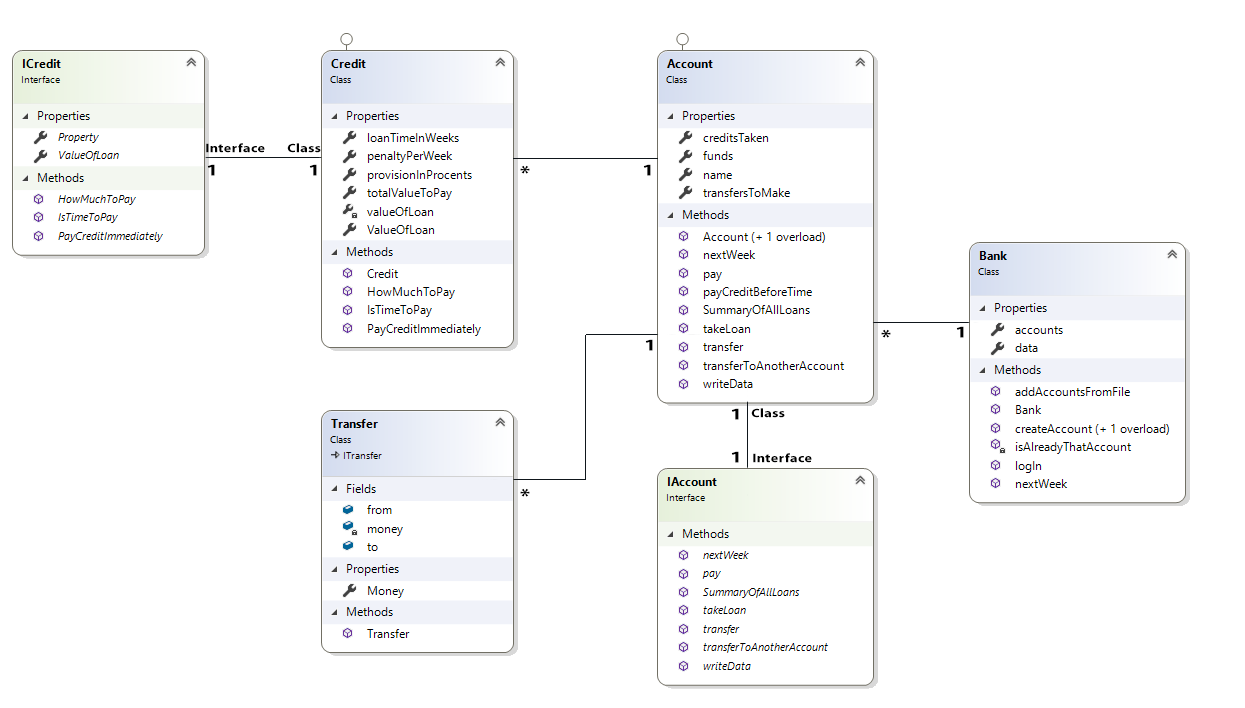
\includegraphics[width=20cm,height=12cm]{ClassDiagram.png}}
\end{center}






\end{document}